% Template for APA submission with R Markdown

% Stuff changed from PLOS Template
\documentclass[10pt, letterpaper]{apa6}
\usepackage{apacite}

% amsmath package, useful for mathematical formulas
\usepackage{amsmath}
% amssymb package, useful for mathematical symbols
\usepackage{amssymb}

% hyperref package, useful for hyperlinks
\usepackage{hyperref}

% graphicx package, useful for including eps and pdf graphics
% include graphics with the command \includegraphics
\usepackage{graphicx}

% Sweave(-like)
\usepackage{fancyvrb}
\DefineVerbatimEnvironment{Sinput}{Verbatim}{fontshape=sl}
\DefineVerbatimEnvironment{Soutput}{Verbatim}{}
\DefineVerbatimEnvironment{Scode}{Verbatim}{fontshape=sl}
\newenvironment{Schunk}{}{}
\DefineVerbatimEnvironment{Code}{Verbatim}{}
\DefineVerbatimEnvironment{CodeInput}{Verbatim}{fontshape=sl}
\DefineVerbatimEnvironment{CodeOutput}{Verbatim}{}
\newenvironment{CodeChunk}{}{}

% cite package, to clean up citations in the main text. Do not remove.
\usepackage{cite}

\usepackage{color}

% Use doublespacing - comment out for single spacing
%\usepackage{setspace}
%\doublespacing


% Text layout
\topmargin 0.0cm
\oddsidemargin 0.5cm
\evensidemargin 0.5cm
\textwidth 16cm
\textheight 21cm

% Bold the 'Figure #' in the caption and separate it with a period
% Captions will be left justified
\usepackage[labelfont=bf,labelsep=period,justification=raggedright]{caption}


% Remove brackets from numbering in List of References
\makeatletter
\renewcommand{\@biblabel}[1]{\quad#1.}
\makeatother


% Leave date blank
\date{}

%\pagestyle{myheadings}
%% ** EDIT HERE **


%% ** EDIT HERE **
%% PLEASE INCLUDE ALL MACROS BELOW

%% END MACROS SECTION


% ALL OF THE TITLE PAGE INFORMATION IS SPECIFIED IN THE YAML
\title{\textbf{Optimal Models for Resource Allocation in Classroom Teaching}}
\shorttitle{}

\author{\large \bf Lawrence Liu}


\authornote{}
\abstract{How should a school administrator allocate a fixed budget towards
increasing the number of classrooms and increasing student assessment to
best increase student learning? This paper investigates how stochastic
models accounting for the inherent uncertainty in student beliefs and
teacher communication can help school administrators figure out how to
maximize student learning by optimally allocating resources. We
replicate existing results from education literature about the effect of
class sizes, homogenous ability classrooms, and assessment on student
learning using computer simulation. We also unify these different
determinants of student learning into a more holistic model and report
the tradeoffs that committing budget to these design features presents,
examining interactions between these constructs not explored and not
feasible in human subjects research. Crucially, we found that sorting
students by ability level is a dominant strategy for improving learning
outcomes. We also report how the effectiveness of class sizes and
assessment is contingent upon the learning concept being taught.
Finally, we demonstrated that we can create a pareto frontier of the
affordable number of teachers and assessments for any budget and
exhaustively explore these configurations to find an optimal allocation
of each budget for increasing student learning. We believe that the
insights about student learning in multi-classroom settings that we've
found and can continue to surface are difficult to surface in real-world
studies with human subjects.}
\keywords{Teaching; learning; education; pragmatics; Bayesian modeling; social
cognition}

\begin{document}
\maketitle

Education research has surfaced many insights into policies for
designing schools to improve classroom learning for students. Very
prominently, conventional wisdom makes independent claims that
decreasing class sizes, increasing formative assessments, and increasing
teaching periods \emph{{[}citation needed for last one{]}} improves
student learning outcomes. However, decreasing class sizes and
developing formative assessments compete for a shared resource of money,
while administering formative assessments and teaching lessons compete
for a shared resource of student time. As such, it is important to
understand the diminishing returns for each of these orthogonal design
dimensions in order to find a unified policy that is optimal for student
learning. We call the optimal policy \textbf{optimal school
administration}.

Unfortunately, there exists many barriers to studying optimal school
administration in real-world classrooms. Isolating the effects of a
chosen school design policy would require controlling for student and
teacher differences, and no two classrooms, teachers, and students are
the same. Even if we could control for these sources of random error,
the task of testing hundreds of permutations across multiple policy
dimensions would be time- and cost-prohibitive, along with being
ethically suspect in some extreme cases. As such, the task of
determining optimal school administration lends itself well to computer
modeling.

In this present paper, we turn to stochastic modeling to investigate how
an optimal school administrator might allocate finite resources to
produce maximal information gain. We elect to utilize stochasticity to
build inherent student variability and error on assessments in the real
world into our model. Taken together, this work describes a
first-principles attempt at a framework for understanding resource
allocation in classroom education.

\section{Background}\label{background}

Even when students are motivated to learn, and teachers are motivated to
teach, information transmission in classroom settings are imperfect.
Education in classroom settings has two challenges that we seek to
tackle. First, there exists a problem of \emph{student variability},
where students within the same classroom may have different innate
academic ability as well as upbringings. This means that a lesson that
would be perfect for one child may be less accessible to another child.
Secondly, there exists a problem of \emph{imperfect teacher knowledge}.
Teachers don't have perfect knowledge of each student's personal
knowledge, and this uncertainty potentially results in choices of
teaching exmaples that are not optimal for student learning.

\subsection{Definitions}\label{definitions}

Because our work builds on some fields of research that have different
vocabularies for similar concepts, we first clarify the language and
meanings that will appear in this paper.

\subsubsection{Types of knowledge}\label{types-of-knowledge}

Every student possesses their own malleable \emph{personal knowledge}
about any knowledge concept, which could be facts, skills, beliefs, or
any other type of knowledge. Coloquially, personal knowledge is often
referred to as \emph{ability level} or \emph{mastery level}, and we use
these terms interchangeably.

Teachers can identify a static \emph{target knowledge} about any
knowledge concept, and a student's personal knowledge can be close to or
far from the target knowledge, representing accuracy or inaccuracy
respectively. The goal of education, therefore, is to adjust the
student's personal knowledge to be as close to the target knowledge as
possible.

Teachers possess beliefs about what their students' personal knowledge
is, which we will call \emph{teacher beliefs}. These may not necessarily
accurately reflect their students' actual personal knowledge.

\subsubsection{Education processes}\label{education-processes}

Assessing, teaching and learning are the three key component processes
of education. \emph{Assessing} involve students providing information to
teachers to \emph{assessments} (e.g.~assignments, quizzes, exams,
classroom participation, etc.) based on their personal knowledge. The
answers provided help teachers update their teacher beliefs.

\emph{Teaching} involves a teacher providing \emph{lessons} to students
to help adjust their students' personal knowledge towards the target
knowledge. The content of the lessons are determined by the teacher
beliefs; in other words, the teacher chooses \emph{teaching examples}
that they believe are most suitable given their students' personal
knowledge.

Finally, \emph{learning} involves a student using the teaching examples
provided by the teacher through teaching to update their own personal
knowledge. Learning itself does not guarantee that a student will update
their personal knowledge to be closer to the target knowledge; the
student must rely on the teacher to pick effective teaching examples for
the updates to be useful.

\subsubsection{Example -- TODO: Keep this
section?}\label{example-todo-keep-this-section}

A teacher wants to teach the effectiveness of nonviolent protest--the
\emph{target knowledge} is that nonviolent protests are somewhere
between always successful and never successful. There is a student who
holds the (inaccurate) \emph{personal knowledge} that nonviolent protest
is always unsuccessful. While there indeed are instances of failed
nonviolent protests (e.g.~Tianenmen Square, The White Rose), a teacher
may elect to over-represent successful nonviolent protests in their
\emph{lessons}, using Martin Luther King Jr., Gandhi, and Nelson Mandela
as \emph{teaching examples}.

\subsection{Related Work}\label{related-work}

\subsubsection{Education Research}\label{education-research}

Educators have a variety of strategies to address the problems of
student variability and imperfect teacher knowledge. Formative
assessments can help teachers monitor their students' personal
knowledge. When students complete formative assessments, teacher gain
certainty on their teacher beliefs about their students' personal
knowledge (e.g., L. S. Fuchs \& Fuchs, 1986; Sadler, 1989). If there is
large variation in students' ability levels, students can be sorted into
groups by teacher beliefs about their personal knowledge and taught
different lessons (e.g. Slavin, 1987; Tomlinson, 1999). Finally,
decreasing class sizes can help minimize the average variation that each
teacher has to deal with in their classroom (e.g., Glass \& Smith, 1979;
Slavin, 1989). Each of these strategies are considered effective ways to
improve student learning.

\subsubsection{Classroom Modeling}\label{classroom-modeling}

In our previous work, we conceptualized the teacher's task as one of
optimal communication (Frank, 2014). Following the models of pragmatic
reasoning in language comprehension (Frank \& Goodman, 2012; Goodman \&
Frank, 2016), we can formalize teaching and learning as inferential
cognitive processes of rational agents. Teachers reason about what
evidence would best change students' personal knowledge to more closely
correspond to a target knowledge. Teachers -- each with perfect teacher
knowledge about each of their students in our prior work -- would then
choose the teaching examples that maximized information gain across
their students. Using this conceptualization, we were able to derive a
number of results through simulation. For example, we found that
individual student outcomes were inversely related to class size, since
in smaller classes, teachers could customize their teaching better to
the idiosynrasies of their particular group of students' personal
knowledge.\footnote{Ability grouping has a complicated history in
  education (e.g., Slavin, 1990), and we return to motivational issues
  related to this finding in the General Discussion.}

In that previous work and the current work, the fundamental unit of
analysis is a teaching game. In each teacher-class unit, a teacher tries
to guide the students to discover a particular target knowledge by
presenting teaching examples. We use a very simple concept: the weight
of a biased coin. The target knowledge is a particular fixed weight, and
the students' personal knowledge was their individual beliefs about what
the weigh tof the coin is. Teachers must choose a particular set of
teaching examples of heads and tails that will alter the personal
knowledge of the students in the class so that their updated estimate of
the coin weight is closer to the teacher's target knowledge value.

\subsection{The Present Study}\label{the-present-study}

In the current work, we consider issues of student variability and
imperfect teacher knowlege through the lens of \emph{optimal school
administration}. We describe a generalization of the model presented in
Frank (2014) and use this framework to investigate how an optimal
adminstrator might make decisions. Our first two simulations replicate
and extend results from the previous paper. Then our next two generalize
the model to the case of imperfect information about students and finite
resources for hiring teachers and conducting assessments. Our final
simulation maps out a Pareto frontier for allocation of instructional
time and teaching resources.

\section{Model}\label{model}

We model three types of agents: \emph{students}, \emph{teachers}, and
\emph{administrators}. A school consists of an administrator, at least
one teacher, and at least one student. Every teacher has at least one
student (so there are always at least as many students as teachers).
Each agent's functions are described below.

The general teaching game that we analyze is one in which learners must
estimate the parameter of a Bernoulli distribution. Teaching lessons are
the results of individual coin flips, which provide evidence about the
coin's weight. Beliefs can then be represented as the parameters of a
Beta distribution. For example, a student who has a weak belief that a
coin is fair (e.g., \(Beta(1,1)\)) can be pursuaded that it is actually
biased towards heads by seeing the examples \(E = \{H, H, H, H, H\}\).

\subsection{Student}\label{student}

Each student is an optimal Bayesian learner, using a standard conjugate
Beta-Bernoulli model. Students each have their own \emph{prior personal
knowledge} about the bias of the coin, represented as
\(Beta(\alpha,\beta)\), where \(\alpha\) and \(\beta\) are
``pseudocounts'' of heads and tails respectively. Students' learning is
then modeled as updating this distribution by adding observed counts to
their priors, e.g.~after observing \(x\) heads and \(y\) tails in the
teaching examples shown by the teacher, their updated \emph{posterior
personal knowledge} state is \(Beta(\alpha + x, \beta + y)\). Note that
for simplicity, student learning is sequence-independent (i.e., seeing
\(\{H, T, T\}\) is the same as seeing \(\{T, T, H\}\)).

Note that student personal knowledge distributions are generated by
sampling \(\alpha \sim Unif(1,10)\) and then setting
\(\beta = 11 - \alpha\) (so that total pseudocounts sum to 11). We
intentionally hold constant the sum of pseudocounts because it controls
how strongly each teaching example affects the student posterior
personal knowledge -- for example, a student who has a prior personal
knowledge distributed as \(Beta(10,10)\) will have their posterior
personal knowledge swayed much more heavily compared to a student whose
prior personal knowledge is distributed as \(Beta(30,30)\) when seein
\({H, H, H, H, T}\).

\subsection{Teacher}\label{teacher}

Each teacher is assigned a classroom of students and a target knowledge
concept (i.e., a particular coin weight) to teach. The goal of the
teacher is to provide the set of teaching examples that maximize the
student's information gain (IG; defined below). This goal is
accomplished by evaluating the information gain for each student for
each possible set of teaching examples and choosing the one that
produces the largest total information gain for the class.\footnote{A
  fruitful direction for future work would be to investigate different
  classroom rules for information gain. For example, a teacher following
  a remedial policy could try to find the set of examples that maximized
  the performance of the lowest-performing students or that minimized
  loss with respect to some threshold.} Since information gain is
computed over the conjugate posterior personal knowledge of the
students, choosing an action relative to IG constitutes full posterior
inference. With only a single teaching example, this choice is simply
the ratio of the IG for \(H\) to the IG for \(T\).

In Simulations 1 and 2, teachers have \emph{perfect teacher beliefs} of
student beliefs. Teachers with perfect teacher beliefs infer their
choice of examples using the exact parameters of student distributions.
In contrast, the teachers in the remaining simulations have
\emph{uncertain teacher beliefs}. Teachers with uncertain knowledge
initially represent students as having beliefs in the form of
\(Beta(1,1)\) -- weak uniform distributions over possible parameter
values. They update these representations based on \emph{assessments}.
For example, if a student was given three assessments and produced
\(\{H, T, H\}\), the teacher would represent that student as
\(Beta(1+2,1+1) = Beta(3,2)\) and choose examples to accordingly.
Assessments are sampled examples from a Bernoulli distribution
parameterized by each student's mean parameter estimate, using
\(\mu = \frac{\alpha}{\alpha + \beta}\). Teachers integrate the samples
from these assessments into their distributional estimate for each
student.

\subsection{Administrator}\label{administrator}

The objective of the administrator is to maximize the information gain
of all students in the school. Across our simulations, the administrator
can decide: 1) how many teachers to hire, 2) how many assessments to
give, and 3) whether to sort students into classrooms by their
knowledge. We also vary (for purposes of comparison) whether the
teachers have perfect or uncertain teacher beliefs of the students'
personal knowledge, though in real-world settings teachers only have
uncertain beliefs. The administrator weights the various policies that
they simulate based on the aggregate information gain of the students in
the entire school (compared to just each classroom for each teacher's
inference), and is able to infer the most effective school design within
fixed constraints. As in the case of teachers, in Simulations 1 and 2,
administrators also have perfect knowledge of their students' personal
knowledge. In contrast, in Simulations 3 and 4, administrators sort
students based on the results of their assessments, the same information
with which teachers use to choose examples.

In practice, because our results demonstrate near-strict dominance of
some design choices over others, the administrator's inference is often
uninteresting and corresponds to the best choice. Thus, in reporting our
simulations, we report school-wide information gain (the decision-making
metric for the administrator), often with respect to some meaningful
baseline.

\subsection{Limited Resources}\label{limited-resources}

In our model, two types of resources restrict the behavior of the
different agents.

\subsubsection{Time}\label{time}

In real-world education settings, students are in a school environment
for a (roughly) fixed amount of time, and it is up to the teachers to
decide what amount of that time they want to dedicate to assessing
(i.e.~formative assessments) and teaching (i.e.~showing teaching
examples). In Analysis 3 and 4, where we use ``noisy'' students,
teachers have the option to assess students to improve their imperfect
teacher beliefs about the students' personal knowledge. We model this
using a resource we call fixed \emph{time steps}. The sum of the number
of \emph{assessment periods} and \emph{teaching periods} is constant,
and increasing assessments comes at the expense of opportunities to show
examples. The administrator commits to a particular allocation of time
steps towards assessments and teaching lessons school-wide, so every
teaacher presents the same number of teaching examples.

\subsubsection{Money}\label{money}

Certain educational policies that may be most effective are simply too
monetarily expensive to implement. For instance, while one-to-one
instruction (i.e.~class sizes of 1) may be most beneficial for student
learning outcomes (e.g., Cohen, Kulik, \& Kulik, 1982), it is
unrealistic to expect schools to be able afford hiring as many teachers
as they have students. To account for this kind of limitation, we
introduce the resource of money into our model. In Simulation 3, the
administrator is constrained by a fixed budget. The cost structure is
described in detail in Simulation 3. We report what the optimal
allocation of money is at every budget level and what the actual
information gain is given that allocation of money.

\subsection{Information gain}\label{information-gain}

Following Frank (2014), we use information gain to quantify student
learning. Formally, we assess the Kullback-Leibler divergence (Cover \&
Thomas, 2012) between student knowledge (\(B_S\)) and the teacher's
target distribution (\(B_T\)) both before and after teaching. The
difference between these quantities gives the student's information gain
for a single example \(e\):

\[IG(e) = D_{KL}(B_T ||B_S) - D_{KL}(B_T || B_{S+e})\]

We derived a closed form expression for information gain that
generalizes to any number of examples in an example set \(e\).
Derivation details can be found in our linked repository. The final form
for \(h\) heads and \(t\) tails is:

\[IG(E) = \sum_{k=0}^{h+t-1} {log(\alpha_S + \beta_S + k)} - \\\]
\[\sum_{i=0}^{h-1} {log (\alpha_S + i)} - \sum_{j=0}^{t-1} {log(\beta_S +j)} + \\\]
\[\psi(\alpha_T)h + \psi(\beta_T)t +  \psi(\alpha_T + \beta_T)(h+t).\]

\noindent where \(\psi\) represents the digamma function, and
\(\alpha_S\), \(\beta_S\), \(\alpha_T\), and \(\beta_T\) are student and
teacher priors respectively.

\subsection{Belief Expectation and Belief
Strength}\label{belief-expectation-and-belief-strength}

As discussed earlier, we represent the target knowledge, student
knowledge, and teacher beliefs about the student knowledge as Beta
distributions \(Beta(\alpha, \beta)\). Frank (2014) presented an
alternative parameterization of the Beta-Bernoulli distribution in terms
of shape \(\mu\) and scale \(\nu\) that is useful for its intuitive
conceptual analogs(Frank, 2014). \(\mu\) and \(\nu\) are defined as:

\[\mu = \alpha / (\alpha + \beta)\] \[\nu = \alpha + \beta\]

In this parameterization, \(\mu\) directly controls the mean of the
distribution. In the target knowledge distribution, this can be regarded
as the \emph{true weight} of the coin. In the student knowledge
distribution, \(\mu\) represents the student's \emph{best guess} for the
true weight of the coin. In the teacher belief distribution, \(\mu\)
represents what the teacher believes the student's best guess for the
true weight of the coin would be (i.e.~given the teacher belief about
the student knowledge). Since Beta-Bernoulli distributions are symmetric
around \(\mu = 0.5\) (e.g.~for the same \(\nu\), the probability
distribution for \(\mu = 0.3\) is the same as \(\mu = 0.7\) flipped
across 0.5), we only look at \(\mu \geq 0.5\), where the true weight or
best guess is more extreme for \(\mu\) values further away from 0.5. In
each case, \(\nu\) captures the \emph{belief strength} or confidence.
The larger \(\nu\) is, the greater the number of examples of Heads or
Tails that would be necessary to alter the belief.

For example, a student with student knowledge \(Beta(5,5)\) and another
student with student knowledge \(Beta(10,10)\) would both have a best
guess that the coin weight is 0.5, i.e. \(\mu\) = 0.5, but fewer
teaching examples would be required to convince the former student that
the true weight actually is not 0.5 than the latter because the former
has weaker beliefs in that \(\mu\) value at \(\nu\) = 10 compared to the
the latter's stronger beliefs at \(\nu\) = 20. Similarly, one students
with student knowledge \(Beta(1,9)\) and another with student knowledge
\(Beta(9,1)\) have vastly different best guesses for the true weight of
the coin (\(\mu\) = 0.1 and \(\mu\) = 0.9 respectively). However,
because both share the same belief strengths at \(\nu\) = 11, their
beliefs about the coin's weight could be shifted to 0.5 with an equal
number examples (8 tails for the former and 8 heads for the latter to
achieve \(Beta(9,9)\)).

\section{Simulations}\label{simulations}

In this section, we present the hypotheses and results of each of our
simulations. Each simulation consists of 100 \emph{trial}s. Each trial
involves generating 100 random students and measuring the aggregate
information gain for those 100 students under the particular school
design policy the simulation is testing. The performance of the school
design policy is calculated as the average of the aggregate information
gain across all 100 trials.

\subsubsection{General simulation
details}\label{general-simulation-details}

All simulations were conducted using the probabilistic programming
language \texttt{WebPPL} (Goodman \& Stuhlmüller, n.d.); the code is
available at {[}\url{http://github.com/mcfrank/teaching}{]}.

In our simulations, there is a set of three parameters that we hold
constant across all experiments for simplicity. While changes to these
parameters will have some impact on the effect sizes we recover, to our
knowledge all qualitative results are general across parameter sets.

\begin{itemize}
\item
  First, the target knowledge is always represented by a Beta
  distribution such that the parameters of \(Beta(\alpha,\beta)\) are
  non-zero and sum to 10, i.e. \(\alpha + \beta = 10\). We choose 10
  because the calculation of the true weight of the coin \(\mu\) are
  simply clean increments of one-tenths. Additionally, because the
  effects would be symmetric if \(\alpha\) and \(beta\) were swapped, we
  restrict \(\alpha <= \beta\). That is, the target knowledge true
  weight is limited to {[}.5, .6, .7, .8, .9{]}.
\item
  Second, the prior student knowledge is always represented by a Beta
  distribution such that the parameters of \(Beta(\alpha,\beta)\) are
  non-zero and sum to 11, i.e. \(\nu = \alpha + \beta = 10\). This fixes
  the belief strength of every student's prior student knowledge --
  every example shown by a teacher will carry the same weight for every
  student because the sum of the pseudocounts is always equivalent. The
  total pseudocounts of prior student knowledge distributions, \(\nu\) =
  11, is slightly offset from the pseudocount of the target knowledge
  distribution, \(\nu\) = 10, to avoid edge cases where a student belief
  distribution perfectly matches the teaching concept.
\item
  Third, each student has 12 learning opportunity time steps. As
  mentioned earlier, each time step can be uesd as a teaching period to
  show examples or, in the relevant simulations, as an assessment period
  to assess students. We choose 12 time steps because it is a sufficient
  number to effectively alter the beliefs of students with extreme prior
  personal knowledge (e.g. \(Beta(1,10)\) can be changed all the way to
  \(Beta(13,10)\)), but does not become computationally prohibitive, as
  WebPPL explores all combinations in its inferences. 
\end{itemize}

\subsection{Perfect Teacher Beliefs}\label{perfect-teacher-beliefs}

In an ideal world, administrators and teachers have perfect teacher
beliefs: they know the exact parameters of each students' personal
knowledge distribution. As such, they can perfectly choose an optimal
set of teaching examples that will maximize the total aggregate
information gain of the students in their classroom. In addition,
administrators can sort students into classrooms by their prior personal
knowledge perfectly -- this ensures that teachers receive classrooms
with as little variance in student personal knowledge as possible,
making it easier to choose sets of teaching examples that are effective
for all students in their respective classrooms. We use such a
simulation environment with perfect teacher beliefs in our first three
simulations (Simulation 1A, 1B, and 1C, details described below).

Running experiments in a simulation environment with perfect teacher
beliefs can be an effective way to uncover the effects of certain
aspects of school design policy because it removes sources of error that
arise from teachers simply not having accurately measured students'
prior personal knowledge. In doing so, we can ascertain that any effects
on information gain are entirely accounted for by the school design
policy. Additionally, in later simulations, we can use the student
information gain outcomes in an environment with perfect teacher beliefs
to benchmark the performance of school design policies in an environment
with imperfect teacher beliefs. The outcomes in the environment with
perfect teacher belief will serve as a strict maximal ceiling or
``gold'' standard -- the dropoff in information gain outcomes in an
imperfect environment we can confidently attribute to inefficiencies
that arise when teachers imperfectly infer students' personal knowledge.

It's worth explicitly noting that teachers having perfect teacher
beliefs does not mean the set of teaching examples that they choose to
use is optimal for each student. In many classrooms, there is no set of
teaching examples that is unanimously optimal at the individual student
level for every student. Rather, having perfect teacher beliefs enables
teachers to pick sets of teaching examples with total certainty that it
will be optimal at the classroom level, and there exists no better set
of teaching examples that would further reduce the inefficiencies of
choosing teaching examples for a varied set of students.

\subsubsection{Simulation 1A: Grouping
students}\label{simulation-1a-grouping-students}

TODO: FIGURE OUT HOW TO LINEBREAK

\begin{CodeChunk}
\begin{figure}[t]
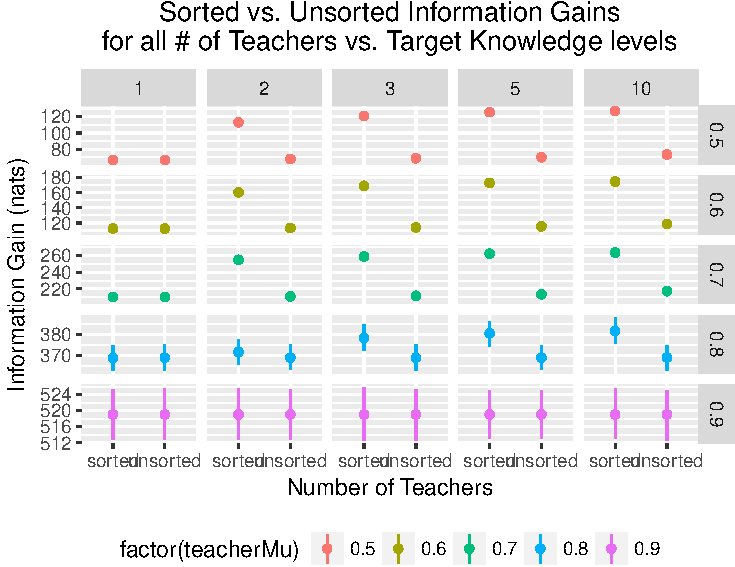
\includegraphics[width=3.25in,height=2.6in]{figs/unnamed-chunk-2-1} \caption[Student information gain, plotted by target concept and number of teachers in the school]{Student information gain, plotted by target concept and number of teachers in the school. Information gain represents the gain when students are sorted into classrooms based on knowledge compared with an unsorted baseline. Error bars show 95\% confidence intervals by non-parametric bootstrap.}\label{fig:unnamed-chunk-21}
\end{figure}
\begin{figure}[t]
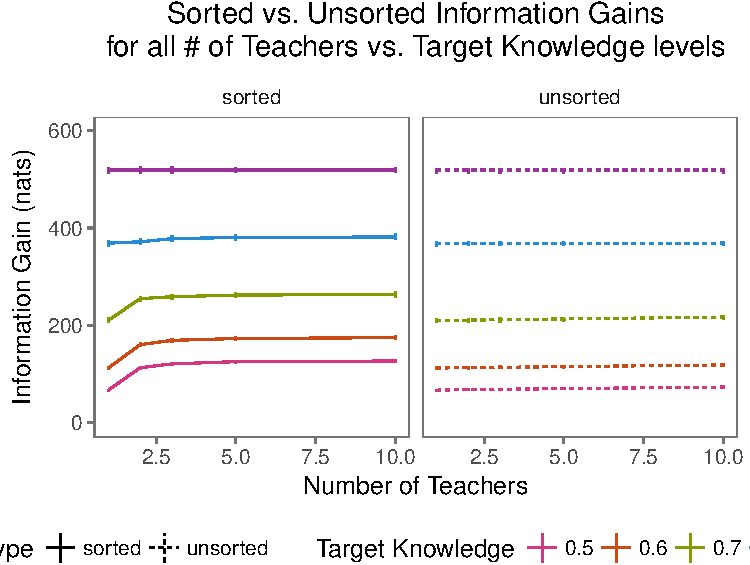
\includegraphics[width=3.25in,height=2.6in]{figs/unnamed-chunk-2-2} \caption[Student information gain, plotted by target concept and number of teachers in the school]{Student information gain, plotted by target concept and number of teachers in the school. Information gain represents the gain when students are sorted into classrooms based on knowledge compared with an unsorted baseline. Error bars show 95\% confidence intervals by non-parametric bootstrap.}\label{fig:unnamed-chunk-22}
\end{figure}
\end{CodeChunk}

\begin{CodeChunk}
\begin{figure}[t]
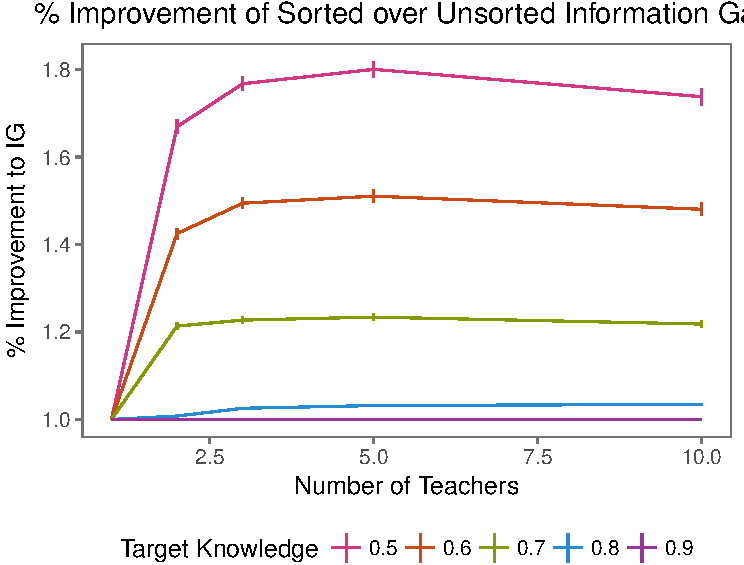
\includegraphics[width=3.25in,height=2.6in]{figs/unnamed-chunk-3-1} \caption[Student information gain, plotted by target concept and number of teachers in the school]{Student information gain, plotted by target concept and number of teachers in the school. Information gain represents the gain when students are sorted into classrooms based on knowledge compared with an unsorted baseline. Error bars show 95\% confidence intervals by non-parametric bootstrap.}\label{fig:unnamed-chunk-3}
\end{figure}
\end{CodeChunk}

\emph{Research Question. } How does grouping students by their true
\emph{prior personal knowledge} affect information gain?

\emph{Design and Hypotheses. } In the manipulation (sorted) condition,
the administrator sorts students into equally-sized (±1 student)
classrooms by their prior personal knowledge. In the control (unsorted)
condition, the administrator performs no sorting, randomly distributing
the students into equally-sized classrooms. We hypothesized that sorting
students by their prior personal knowledge would increase information
gain compared to random classroom assignment because sorting would
reduce variance in student personal knowledge within classrooms,
allowing teachers to better tailor the teaching examples to that
particular group of students.

We further hypothesized that there'd be an interaction effect between
sorting and both the number of teachers and the extremity of the target
knowledge concept. Specifically, we believe that sorting results in
greater information gain as the number of teachers increases, since no
matter how sorted the rosters are, having too many students in one class
still prevents teachers from finding a set of teaching examples that
will be effective for every student in the class. On the other hand, we
believe sorting will be less effective for more extreme target knowledge
concepts (higher \(\mu\) values for the target knowledge distribution),
since for extreme target knowledge concepts, most students will have
best guesses that fall on the same side of the true weight of the coin,
and so no matter what the prior personal knowledge distributions of the
stduents are, the teacher can simply choose very biased teaching
examples and they will be effective.

\emph{Results. } Results are shown in Figure 1. Sorted students show
greater information gain than if the same set of students are
distributed into unsorted classrooms. This effect is present for all
target concepts but is most pronounced for less-extreme concepts -- for
extreme value concepts (e.g., a target of .9), almost all students will
benefit from seeing the same examples anyway, rendering sorting
irrelevant. Thus, an optimal school administrator with perfect student
knowledge should consistently opt to sort students into classrooms by
their prior beliefs over random assignment.

\subsubsection{Simulation 1b: Number of Teachers or Class
Size}\label{simulation-1b-number-of-teachers-or-class-size}

LINEBREAK

\begin{CodeChunk}
\begin{figure}[t]
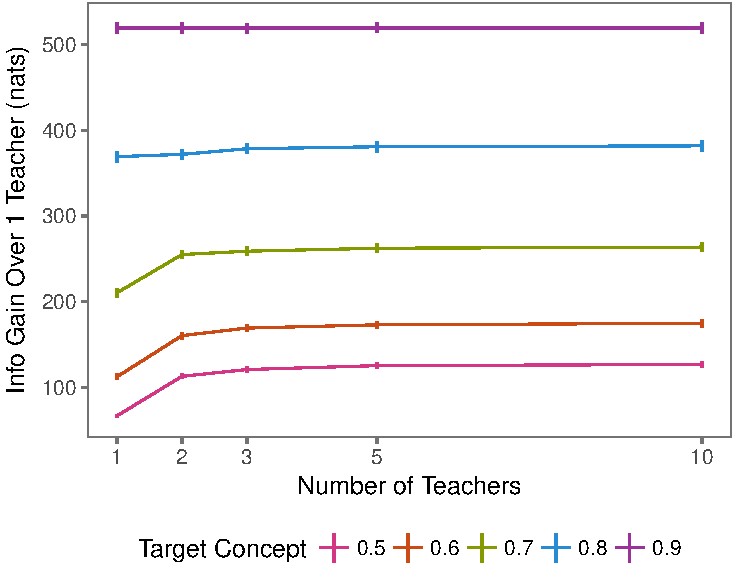
\includegraphics[width=3.25in,height=2.6in]{figs/unnamed-chunk-5-1} \caption[This figure should probably go in the appendix, but helps illustrate why using the baseline is useful]{This figure should probably go in the appendix, but helps illustrate why using the baseline is useful}\label{fig:unnamed-chunk-5}
\end{figure}
\end{CodeChunk}

\begin{CodeChunk}
\begin{figure}[t]
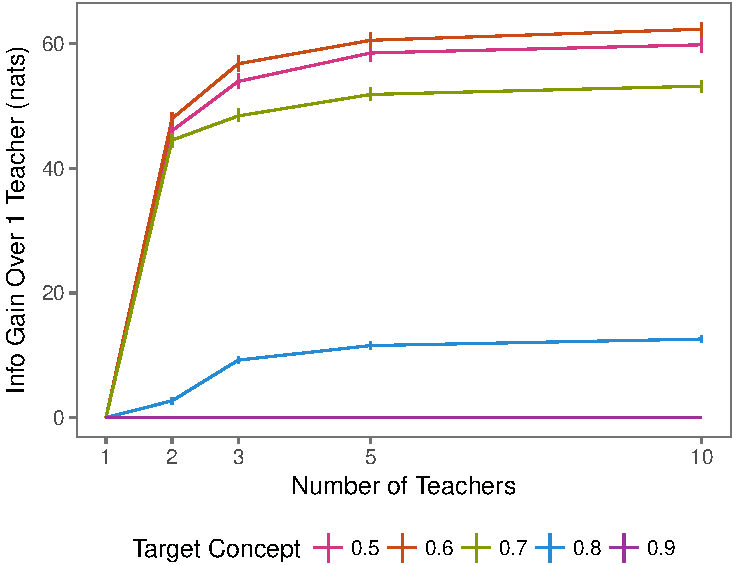
\includegraphics[width=3.25in,height=2.6in]{figs/unnamed-chunk-6-1} \caption[Student information gain, plotted by target concept and class size]{Student information gain, plotted by target concept and class size. Information gain represents the gain when students are sorted into classrooms based on knowledge compared with a single-classroom baseline. Error bars show 95\% confidence intervals by non-parametric bootstrap.}\label{fig:unnamed-chunk-6}
\end{figure}
\end{CodeChunk}

\emph{Research Question. } How does the number of teachers, which is
inversely proportional to the class size, affect student information
gain?

\emph{Design and Hypotheses. } In this simulation, the administrator
changes the number of classrooms to distribute students. There can be 1,
2, 3, 5, or 10 classrooms, resulting in class sizes of 100, 50, 33/34,
20, and 10 respectively. We hypothesized that increasing the number of
teachers would strictly improve student learning rate: just like with
sorting, more teachers would reduce class sizes, which in turn reduces
student variance within classrooms. This enables teachers to choose
better tailored sets of learning examples.

\emph{Results. } Results are shown in Figure 2. We observed the
predicted pattern. Increasing the number of teachers increases the
information gain. although there were diminishing returns. After a
certain number of teachers, additional lesson customization becomes less
helpful.

In our second analysis, again a replication of our prior work, we
explored the effects of adding teachers to the simulated school, leading
to lower class sizes. We hypothesized that increasing the number of
teachers would strictly improve student learning rate (again assuming
perfect knowledge about students): Our baseline for this analysis was
the sorted information gain under the same target bias parameters.

\subsection{Imperfect Teacher Beliefs}\label{imperfect-teacher-beliefs}

In our second set of analyses, we relax the assumption that teachers
have perfect teacher beliefs about students' prior personal knowledge.
In the real world, neither the admin nor the teacher is an omniscient
being that knows the true prior personal knowledge parameters. Instead,
they diagnose student beliefs by administering formative assessments
(e.g.~placement exams). The assessment phase is a necessary step that
enables the administrator and teachers to form teacher beliefs about
what the students' prior personal knowledge may be -- these beliefs are
not perfect, but will be correlated with the students' personal
knowledge. Only after these assessments are conducted can the
administrator effectively sort students. The teachers can also then
select examples guided by these teaching beliefs.

To model these agent behaviors, we assume that the admin and teachers
start with teacher beliefs that are a na"ive, uniform representation of
each student (i.e. \(Beta(1,1)\)) and learn about the student's prior
personal knowledge via the administration of assessments. In
assessments, students are called upon to demonstrate their knowledge by
sampling from their own true prior personal knowledge distribution.
These samples then serve to update the teacher's estimate about student
knowledge. In this sense, the teachers and the administrator are modeled
as perfect Bayesian agents that update their teacher beliefs about
student personal knowledge based on evidence it sees from student
performance on assessments.

For instance, a student may have a true prior personal knowledge
distribution represented by \(Beta(9,2)\). When assessed, they are
extremely likely to respond with \(H\) (or \(1\)) to each question on
the assessment. If they are asked 6 questions, the most common outcome
will be \({H, H, H, H, H, T}\) (in some order). The teachers and
administrator starts with the naive \(Beta(1,1)\) representation of the
student personal knowledge, but then updates the representation for
seeing 5 heads and 1 tail in the assessment phase. Their \emph{posterior
teacher belief} (i.e. (post-assessment) of student learning becomes
\(Beta(6,2)\) after the Bayesian update. By construction, our uncertain
teachers have very weak and inaccurate beliefs about student personal
knowledge, captured by the low \(\nu\) of the initial Beta
representation, and we assume that increasing assessments will help them
improve the accuracy and belief strength of their representation of
student personal knowledge.

Given our model, increasing the number of assessments should
monotonically improve student learning on average because the teachers
get more accurate and precise teacher beliefs about the students' prior
personal knowledge through assessments. As such, simply measuring
information gain as the number of assessments increases is rather
trivial. In the following simulation, we introduce the limited resource
of time--each student spends a fixed number of 12 time steps in the
school system, and any single time step can be devoted to assessing the
student (3 samples from the student's prior persanal knowledge
distribution, as described above) or a teacher showing the student one
teaching example (a heads or a tails). By modeling the tradeoff between
increasing assessments and increasing teaching opportunities, we attempt
to identify a tipping point at which giving teachers more opportunities
to show examples outweight the diminishing returns on information gain
of increasing assessments, and vice versa.

In a simulation environment where imperfect teacher beliefs exist,
inefficiencies are introduced in two ways. First, administrators may
commit errors in sorting students into classrooms if they have an
inaccurate guesses about the mean of students' prior personal knowledge
distributions. Secondly, teachers may choose less efficient sets of
teaching examples based on their guesses about their students' prior
personal knowledge that may not actually optimally maximize information
gain given the students' true prior personal knowledge.

Our previous work on modeling classroom dynamics (Frank, 2014) did not
have any stochasticity in the generation of student distributions nor
the inferences that teachers make about students' prior personal
knowledge. We believe that by capturing the errors in the inferences and
the formative assessments that teachers might use to reduce those errors
in our model, our simulations are a novel contribution to the literature
that more accurately resembles real-world classroom dynamics.

\subsubsection{Baseline}\label{baseline}

In Simulation 1a-1c, we observed that the information gain values vary
significantly across different target knowledge concepts, or the true
weight of the coin \(\mu\). In real-world classroom settings, the target
knowledge concept is an independent variable that are entirely
orthogonal to the school design tradeoffs we are considering -- if high
school students are trying to learn trigonometry, trigonometry must be
the target knowledge regardless of whether its few or many teachers
teaching, regardless of whether or not the students are sorted by
ability level, and regardless of whether few or many formative
assessments are conducted. As such, we want to control for the target
knowledge concept by measuring \emph{improvement} to information gain
\emph{within} levels of the target knowledge concept.

To do so, we introduce a baseline paradigm that uses a non-inferential
admin and teacher that we consider the control condition. The baseline
design involves no student sorting, using a single teacher, and no
assessments (i.e.~12 teaching examples). This admin and teacher does not
take their students' prior beliefs into consideration. Instead, they
simply sample a Binomial distribution with a bias equal to the \(\mu\)
value from the target knowledge distribution to generate their example
sets -- this is equivalent to actually flipping a coin of the weight
\(\mu\). As such, there would be a unique average baseline for each
level of the target knowledge concept, but otherwise utilize the most
basic design along the sorting, number of teachers, and number of
assessments dimensions. We call this baseline control condition the
\emph{naive teacher} policy.

For instance, to generate 12 examples when the target knowledge concept
is 0.7 in any one trial, the teacher would sample from
\(Binomial(n=12, p=0.7)\), with 9 Heads and 3 Tails being most likely, 8
Heads and 4 Tails being next most likely, and so forth. They would then
show this set of teaching examples to every student in their classroom
without consideration for their prior personal knowledge and whether or
not that teaching example would actually be useful given their prior
personal knowledge.

\subsubsection{Simulation 2: Imperfect Teacher
Beliefs}\label{simulation-2-imperfect-teacher-beliefs}

As we consider imperfect teacher beliefs, we attempt to unify some of
the different dimensions from Simulation 1 of sorting vs.~unsorting, and
the number of teachers while incorporating the new dimension of the
number of assessments. Each of these dimensions may interact with the
other, and so unlike in Simulations 1a-1c, we first report the full set
of results before we slice the dataset and discuss each dimension in
greater detail.

\begin{CodeChunk}
\begin{figure*}[t]
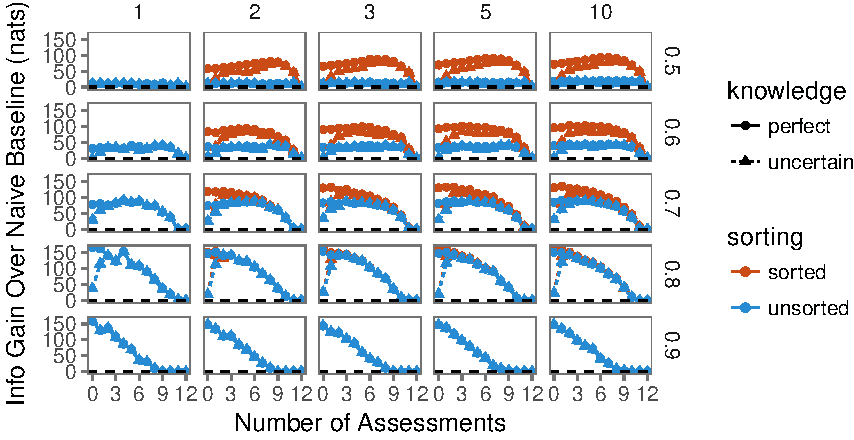
\includegraphics[width=3.25in,height=2.6in]{figs/sim_noisy_students-1} \caption[Information gain plotted by number of assessments (out of 12) for teachers with perfect and uncertain student knowledge]{Information gain plotted by number of assessments (out of 12) for teachers with perfect and uncertain student knowledge.}\label{fig:sim_noisy_students}
\end{figure*}
\end{CodeChunk}

\begin{CodeChunk}
\begin{CodeInput}
#TODO: Determine if this needs to be in there.
df_lm <- ig_by_sim_type %>%
  separate(sim_type, into = c("sorting","knowledge"))

model <- lm(IG_over_baseline ~ numTeachers + sorting * teacherMu * numAssessments, df_lm)
\end{CodeInput}
\end{CodeChunk}

\subsubsection{Simulation 2a: Sorting}\label{simulation-2a-sorting}

LINEBREAK

\emph{Research Question. } Do the effects of sorting students by their
prior personal knowledge found in Simulation 1a persist when the
teachers have imperfect teacher knowledge? How do the effects compare
with when the teachers have perfect teacher beliefs?

\emph{Design and Hypotheses. } We use a 2 (sorted vs.~unsorted) x 2
(perfect vs.~imperfect teacher beliefs) experimental design. The sorted
x perfect condition and unsorted x perfect condition are a replication
of Simulation 1a's manipulation and control conditions respectively. In
the sorted x imperfect condition, the administrator sorts students into
equally-sized (±1 student) classrooms by the \emph{teacher beliefs}
about the prior personal knowledge, which are correlated with the prior
personal knowledge itself due to the assessment phase but not
necessarily identical. In both the sorted and unsorted imperfect
conditions, teachers choose teaching examples that would be optimal
given the teacher beliefs about the prior personal knowledge.

We hypothesized that sorting students into classrooms using imperfect
teacher beliefs would still result in greater information gain than
random student assignments. However, we suspected that the information
gain achieved after sorting with imperfect teacher beliefs would be
lower than when the students were sorted by their true prior personal
knowledge because there may be sorting errors when using the imperfect
teacher beliefs.

\emph{Results. } As we predicted, sorting students produced a main
effect on learning outcomes that were strictly superior than not sorting
in both the perfect teacher belief condition (consistent with Simulation
1a) as well as the imperfect teacher belief condition. Just as in
Simulation 1a, the effect of sorting interacts with number of teachers,
where sorting has no effect when there is only 1 teacher because there
is only 1 classroom (leftmost column in Figure 4). Similarly, the effect
of sorting also interacts with target knowledge concept as it did in
Simulation 1a, where sorting becomes less effective for more extreme
target knowledge concepts (greater difference between red sorted IGs and
blue unsorted IGs the higher the row in Figure 4).

Perhaps surprisingly, sorting students by the imperfect teacher beliefs
still vastly outperforms unsorted school designs even when the teachers
have perfect teacher beliefs and can pick the most optimal teaching
examples within classrooms. This underscores the dominance of sorting
policies. Without sorting, no matter how much an administrator increases
the number of teachers or or assessments, students do not appear to gain
substantially more information, because each classroom on average is
still a representative microcosm of the entire set of students.

Given these results, we assume the optimal school administration policy
uses student sorting, and we discuss all subsequent simulation analyses
in terms of their information gain when students are sorted.

\subsubsection{Simulation 2b: Number of Teachers / Class
Size}\label{simulation-2b-number-of-teachers-class-size}

LINEBREAK

\emph{Research Question. } Do the effects of the number of teachers by
their prior personal knowledge found in Simulation 1b persist when the
teachers have imperfect teacher knowledge? How do the effects compare
with when the teachers have perfect teacher beliefs?

\emph{Design and Hypotheses. } We use a 5 (1, 2, 3, 5, and 10) x 2
(perfect vs.~imperfect teacher beliefs) experimental design. Based on
our results from Simulation 1b, we hypothesized that increasing the
number of teachers would strictly improve student learning rate because
each classroom will be smaller, allowing teachers to pick more tailored
teaching examples for their classroom. We also hypothesized that the
improvement to information gain would have diminishing returns as the
number of teachers increases, just as we found in Simulation 1b. We
further suspect that the effect of increasing the number of teachers
interacts with the extremity of the target knowledge concept. We believe
more extreme target knowledge concepts would benefit less from
increasing the number of classrooms since most students will fall on the
same side of very heavily biased target knowledge concepts.

\emph{Results. } As predicted, increasing the number of teachers
increases the information gain with diminishing returns as the number of
teachers increases. Specifically, we observe that there is a massive
improvement to learning outcomes going from 1 teacher to 2 teachers
especially for more moderate target knowledge concepts of 0.5, 0.6, and
0.7, and smaller and smaller improvements as additional teachers are
used. As expected, having more classrooms does not particularly help
teachers teach extreme target knowledge concepts, as there is no
difference between few and many teachers all showing mostly Heads.

\subsubsection{Simulation 2b: Number of Teachers / Class
Size}\label{simulation-2b-number-of-teachers-class-size-1}

LINEBREAK

\emph{Research Question. } Do the effects of the number of teachers by
their prior personal knowledge found in Simulation 1b persist when the
teachers have imperfect teacher knowledge? How do the effects compare
with when the teachers have perfect teacher beliefs?

\emph{Design and Hypotheses. } We use a 5 (1, 2, 3, 5, and 10) x 2
(perfect vs.~imperfect teacher beliefs) experimental design. Based on
our results from Simulation 1b, we hypothesized that increasing the
number of teachers would strictly improve student learning rate because
each classroom will be smaller, allowing teachers to pick more tailored
teaching examples for their classroom. We also hypothesized that the
improvement to information gain would have diminishing returns as the
number of teachers increases, just as we found in Simulation 1b. We
further suspect that the effect of increasing the number of teachers
interacts with the extremity of the target knowledge concept. We believe
more extreme target knowledge concepts would benefit less from
increasing the number of classrooms since most students will fall on the
same side of very heavily biased target knowledge concepts.

\emph{Results. } As predicted, increasing the number of teachers
increases the information gain with diminishing returns as the number of
teachers increases. Specifically, we observe that there is a massive
improvement to learning outcomes going from 1 teacher to 2 teachers
especially for more moderate target knowledge concepts of 0.5, 0.6, and
0.7, and smaller and smaller improvements as additional teachers are
used. As expected, having more classrooms does not particularly help
teachers teach extreme target knowledge concepts, as there is no
difference between few and many teachers all showing mostly Heads.
Again, we note that this effect only exists with a sorted school policy;
without sorting, increasing the number of classrooms does not guarantee
a significant drop in within-classroom variance in student personal
knowledge.

\subsubsection{Simulation 2c: Number of Assessments vs.~Number of
Teaching
Examples}\label{simulation-2c-number-of-assessments-vs.number-of-teaching-examples}

LINEBREAK

\emph{Research Question. } How do the number of time steps dedicated to
assessment periods vs.~teaching periods affect information gain? If
there exists an effect, does it interact with the number of teachers or
the target knowledge concept?

\emph{Design and Hypotheses. } We use a 13 (0 through 12 assessment
periods) x 5 (1, 2, 3, 5, or 10 teachers) x 5 (0.5 through 0.9 target
knowledge concept) design. In the 12 different time steps, teachers can
either elect to conduct a formative assessment or present a teaching
example (details described earlier). For the sake of simplicity, every
teacher conducts the same number of assessments and shows the same
number of examples, and all assessments must come before the teaching
examples.

We first hypothesized that across all numbers of assessments, there will
be less information gain with imperfect teacher knowledge than with
perfect teacher knowledge due to errors in sorting and non-optimal
teaching example selection.

Next, we hypothesized that there would be a concave down shape in the
effect that manipulating the number of assessments has on information
gain. We thought that a few assessments would get the estimated beliefs
about student knowledge close enough to the students' true beliefs to
minimize sorting errors, leaving teachers with enough time to teach
lessons to move the students' actual beliefs towards the target concept.
Too many assessments would reduce the amount of time teachers have to
teach regardless of how precise their estimates of student knowledge
are; too few assessments would prevent teachers from selecting helpful
examples in their lessons. At one extreme, with no assessments, the
adminstrator and teachers would have no knowledge of the students' prior
personal knowledge to base their sorting into classrooms and selection
of teaching examples on, resulting in arbitrary blind guessing about
which classroom a student should be grouped into and which teaching
examples would be most effective. At the other extreme, if the students
are assessed all 12 time steps, no matter how accurate the teacher
beliefs may be, there are no opportunities to actually show teaching
examples to shift the students' personal knowledge, so the students'
prior and posterior personal knowledge distributions are identical and
there is no improvement over the baseline.

We further hypothsized that this effect would interact with the number
of teachers, where having a the optimal number of assessments for
increasing information gain would be particularly high for more teachers
because having more classrooms should demand more accurate sorting.
Finally, we hypothesized that the effect of assessments would interact
with the extremity of the target knowledge concept (i.e.~the true weight
of the coin), where more extreme target knowledge concepts would have a
lower optimal number of assessments. We suspected that extreme targets
require fewer assessments to accurately discern which classroom a
student belongs in, since most students will require the same set of
teaching examples to reach extreme target knowledge concepts anyway.

\emph{Results. } As predicted, we continue to find that with imperfect
teacher beliefs, teachers perform strictly worse in any given regime of
number of teachers, target knowledge concept, and assessment parameters.
We also found the hypothesized concave down relationship between the
number of assessments and information gain for target knowledge concepts
between 0.5 and 0.8. We also see support for the hypothesized
interaction the target knowledge concept, where higher target knowledge
concepts have a lower optimal number of assessments. We did not find
evidence of the hypothesized interaction between assessments and number
of teachers.

These non-linear results hint at an interesting tradeoff between
assessments and teaching. When there is a moderate target knowledge
concept, the average distance to the target knowledge concept is lower
than when there is an extreme target knowledge concept, and students can
fall on either side of the target. This favors conducting more
assessments for two reasons. First, it is more important to have high
accuracy in the assessment phase to discern whether students' best guess
of the weight of the coin based on their prior personal knowledge falls
below or above the target knowledge concept. Secondly, there is less
teaching to be done because fewer teaching examples are necessary to
calibrate the students' personal knowledge to be close to the target
knowledge. When the target is extreme, you may need many more teaching
examples in order to calibrate a student who has a very distant best
guess (e.g.~0.1) to the extreme target (e.g.~0.9), and you do not need
to precisely measure the students' best guess (e.g.~is it 0.1 or 0.2 or
0.3?) to know that you must show many heads.

This is consistent with the seemingly aberrant results for a target
knowledge concept of 0.9. With such an extreme target concept, no
assessment is even necessary between 1 through 5 teachers to know that
you will be showing mostly Heads regardless of the students' prior
personal knowledge distributions. Only when there are 10 teachers will
there be a class of students who may all consistently benefit from
seeing tails because they fall at or above 0.9 in their own prior
personal knowledge. As such, there is asymptotic behavior as the number
of assessments increases, because the improvement over the baseline
approaches zero.

\begin{CodeChunk}
\begin{figure}[t]
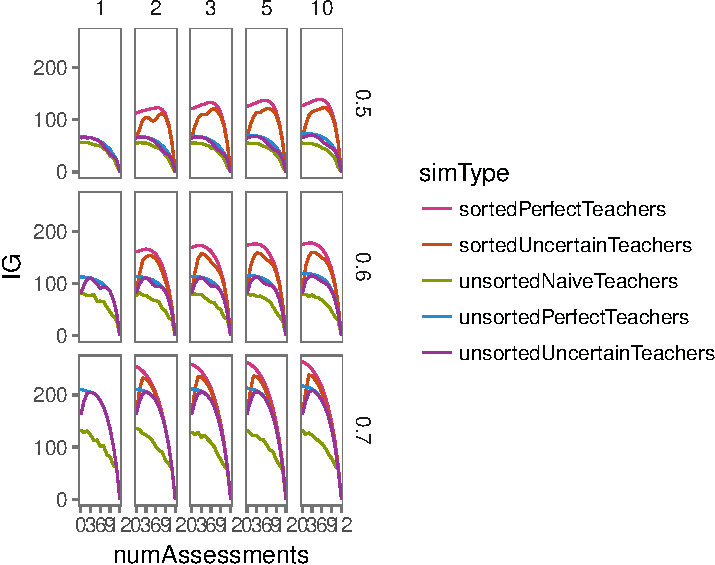
\includegraphics[width=3.25in,height=2.6in]{figs/unnamed-chunk-9-1} \caption[Might be good for showing how sortedPerfect and naive provide upper and lower bounds for the unsortedUncertain teachers]{Might be good for showing how sortedPerfect and naive provide upper and lower bounds for the unsortedUncertain teachers}\label{fig:unnamed-chunk-9}
\end{figure}
\end{CodeChunk}

\subsection{Simulation 3: Pareto frontier with imposed budget
constraints}\label{simulation-3-pareto-frontier-with-imposed-budget-constraints}

LINEBREAK

\begin{CodeChunk}
\begin{figure}[t]
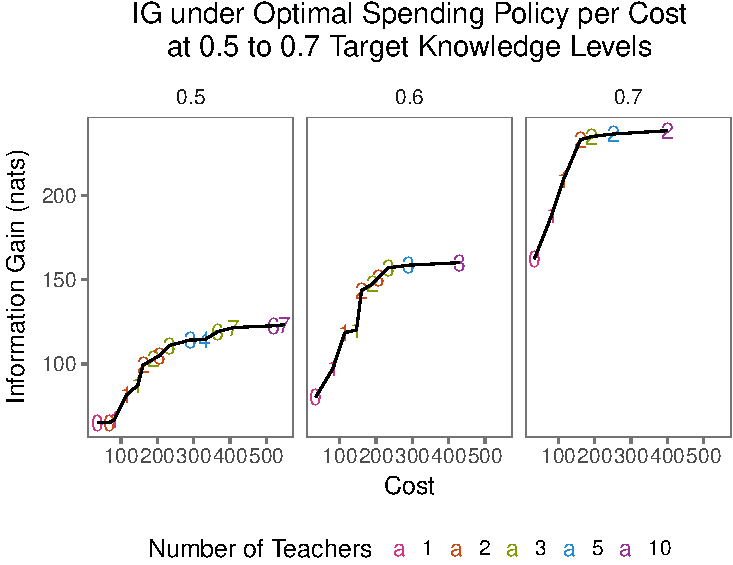
\includegraphics[width=3.25in,height=2.6in]{figs/unnamed-chunk-11-1} \caption[Optimal]{Optimal}\label{fig:unnamed-chunk-11}
\end{figure}
\end{CodeChunk}

\begin{CodeChunk}
\begin{figure}[t]
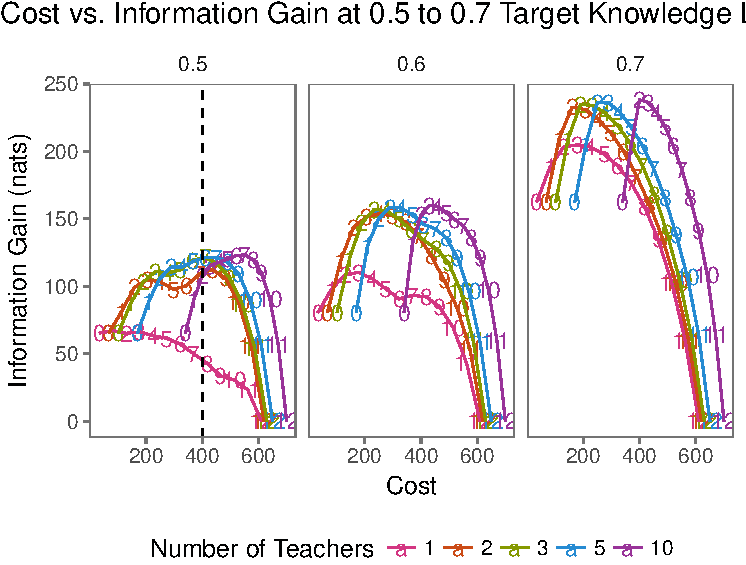
\includegraphics[width=3.25in,height=2.6in]{figs/unnamed-chunk-12-1} \caption[Pareto frontiers]{Pareto frontiers}\label{fig:unnamed-chunk-121}
\end{figure}
\begin{figure}[t]
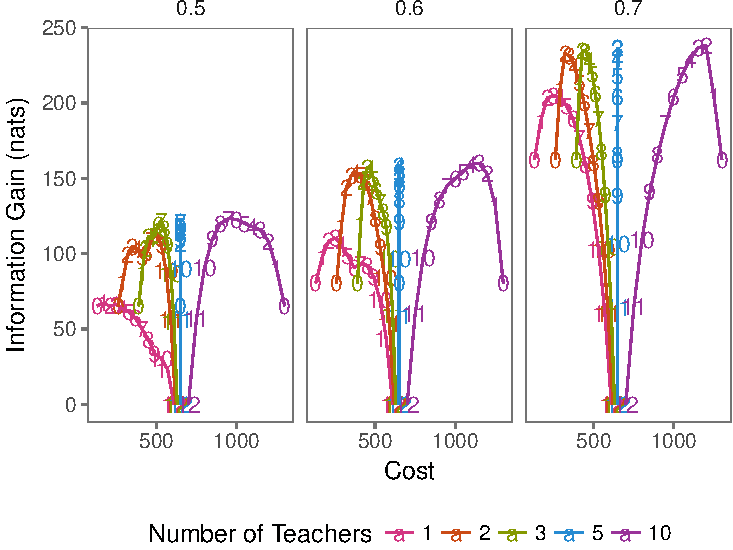
\includegraphics[width=3.25in,height=2.6in]{figs/unnamed-chunk-12-2} \caption[Pareto frontiers]{Pareto frontiers}\label{fig:unnamed-chunk-122}
\end{figure}
\end{CodeChunk}

\emph{Research Question. } How does information gain vary by their cost?
What does the pareto frontier at any cost level look like?

\emph{Design and Hypotheses. } The first model design step was to define
the heuristics for our cost structure. These were the heuristics that we
wanted our cost structure to abide by and the reasoning behind them:

\begin{itemize}
\item
  Each assessment has a fixed cost \(C_A\) independent of the number of
  teachers. In the real world, there is a fixed cost of designing each
  assessment (e.g.~writing a standardized test). Additionally, there is
  the fixed cost of administrating an assessment. This is a fixed cost
  because the environment under which an assessment is administered to
  the students (e.g.~a standardized test in a classroom with a faculty
  member monitoring for academic integrity) is not affected by the
  number of teachers hired to actually teach lessons. We jointly
  consider these as a single fixed cost of each assessment \(C_A\).
\item
  Teachers should receive greater compensation for teaching more
  teaching periods (i.e.~showing more teaching examples). Though our
  model uses a highly simplified lesson, in the real world, a lesson
  could involve lesson planning, preparing teaching materials, providing
  feedback, etc. For every teaching example, each teacher will receive
  an additional \(C_E\) in compensation.
\item
  Hiring each teacher has a fixed cost \(C_T\). Regardless of the number
  of lessons a teacher ends up teaching, there should be some overhead
  cost of interviewing a teacher, one-off training and professional
  development programs, stocking their classroom with school supplies,
  utilities, etc. Hiring 10 teachers to teach 1 lesson each should cost
  more than hiring 5 teachers to teach 2 lessons each.
\end{itemize}

Thus, given \(A\) assessments administered school-wide, \(T\) teachers
hired, and \(E\) time periods dedicated showing teaching examples in
teaching periods, the total cost \(C\) of the school design policy is
\(C = A * C_A + T * (C_T + C_E * E)\). (Recall that the number of
assessment periods is inversely proportional to the teaching periods by
construction due to the limited resource of time. \(E\) could be
rewritten as \(12 - A\), but we use the unique variable \(E\) for
clarity.)

We hypothesize that overall, if money is being spent optimally, spending
more money will produce better learning outcomes but with diminishing
returns because we saw in our earlier simulations that while hiring more
teachers will improve information gain, each additional teacher results
in much smaller improvements to information gain. We further hypothesize
that with an infinite budget, hiring more teachers is trivially most
effective but at smaller cost levels, the pareto frontier involves a
moderate number of assessments and a moderate number of teachers;
neither hiring more teachers nor conducting more assessments is
necessarily always the most effective way to improve information gain.

\emph{Results. } As predicted, information gain increases over time
under optimal spending policies with massive diminishing returns (Figure
8). Additionally, as predicted, we found that the optimal policy at any
smaller budget level within any target knowledge concept level
frequently involved a moderate number of assessments and teachers. For
instance, at the target knowledge \(\mu = 0.5\) level, with \$400
(Figure 9, dashed vertical line), you could afford hiring 10 teachers if
you only have 2 assessment periods, but having only 3 teachers and 6
assessment periods or having 5 teachers with 7 assessment periods both
produced superior information gain outcomes for the same \$400 cost.

We importantly observe that smaller budgets approach the apparent global
optimal information gain much more quickly (see Figure 8). when teaching
extreme target knowledge concepts (visually, this is represented by how
low a cost the information gain plateau begins). As we saw in Simulation
1b and 2b, hiring more teachers is only useful when there is a need for
different classrooms to show different sets of teaching examples, and
that need only exists with moderate (closer to \(\mu = 0.5\)) target
knowledge concepts since with extreme target concepts many teachers end
up showing the same sets of examples anyway. Hiring teachers is
extremely expensive and offer little improvement to information gain
outcomes at extreme target knowledge concepts, so doing so becomes an
inefficient use of money.

Of course, \(C_A\), \(C_T\), and \(C_E\) would vary in the real world
(e.g.~respectively by subject matter, cost of living, and minimum wage).
Our goal is not to advise a definitive number of teachers and
assessments, but rather to point out qualitative effects after
controlling for those costs. To do so, we acknowledge that we pick
arbitrary costs, but to the authors' knowledge the qualititative results
are true for every reasonable choice of costs. Figures 8 and 9 show
results using \(C_A = 50\), \(C_T = 10\), and \(C_E = 2\), but the
appendix contains a few graphs of optimal spending curves and pareto
frontier lines for different costs.

\section{Discussion}\label{discussion}

\subsection{Summary}\label{summary}

Our research sought to create a stochastic model of a classroom
environment in which we can explore how different school design policies
affects student information gain. In our simulations, a school consisted
of an administrator, at least one teacher, and 100 students with
randomly generated ability levels, and the fundamental unit of learning
involves learning the weight of a biased coin. Each agent is a perfect
Bayesian actor that performs inferences on the behavior of other agents
in the system. The administrator chooses how to distribute students into
classrooms, and then teachers selecting teaching examples that they
think will best calibrate students' personal knowledge towards the
target knowledge concept, a process that generates \emph{information
gain}. A particular school design is considered more effective if it
produces greater aggregate information gain.

In education literature, school design dimensions of sorting, number of
teachers or class size, and assessments and their effects on learning
outcomes have only been considered in isolation. Our simulations attempt
to exhaustively consider all combinations of these three dimensions,
ultimately spanning 2 (perfect teacher knowledge vs imperfect teacher
knowledge) x 2 (sorting vs.~not sorting students into classrooms by
ability level) x 5 (1, 2, 3, 5, or 10 teachers) x 5 (0.5 to 0.9 target
knowledge concepts) x 13 (0 to 12 assessment periods) = 1300 different
school design configurations. We perform 100 trials of each
configuration, testing their efficacy at improving information gain on
100 students each time. In total, our full experimental design required
13,000,000 students. While our model simplifies a lot of aspects of
teaching, we believe that if we can reproduce classroom dynamics from
real-world settings, our virtual model empowers us to explore the
interactions that these different constructs have on each other that
would be impossible to test with human subjects and real-world
classrooms.

In order to validate that our model behaves comparably to real-world
education settings, we first replicated some findings that exist in the
education literature. In Simulations 1a and 1b, we use our simplest
model where we have an ``omniscient'' administrator and teachers with
\emph{perfect teacher beliefs}--that is, they know every students' prior
personal knowledge distributions with perfect accuracy. Though this
simple model ignores inherent human errors in knowledge, communication,
and inference, it validated the information theory behind our model and
replicate findings from (Frank, 2014), which used the change in the
Kullback-Leibler divergence between the student's personal knowledge and
the target concept pre- and post-lesson as the measure of information
gain. In these simulations, we were able to replicate real-world
findings that sorting students into ability-level classrooms improves
information gain (Simulation 1a), and increasing the number of teachers
decreases class sizes and improves information gain with diminishing
returns for higher numbers of additional teachers (Simulation 1b). Both
of these main effect interacted with the extremity or difficulty of the
target knowledge concept, where the effects were stronger for moderate
targets and weaker for extreme targets.

Having validated the information theory in our model, we then novelly
introduce stochastic processes into our model to simulate inherent noise
in real-world classrooms. Despite introducing sources of error that
represents student human error during formative assessments,
administrator error in sorting students by ability level, and teacher
error in choosing effective teaching examples, we were again able to
replicate many findings from education literature. In simulation 2a, we
again found that sorting students into ability-level classrooms
significantly improves information gain. In Simulation 2b, we again
found that increasing the number of teachers to reduce class sizes
improves information gain. Again, each of these effects interacted with
the extremity of the target knowledge concept, where each effects was
more pronounced for moderate targets.

In Simulation 2c, introduced the fixed resource of time. We forced
teachers to choose between assessing and teaching students, since both
of those occupy students' limited amount of time in school. Consistent
with past education literature, we found that formative assessments help
administrators and teachers better understand what each students'
ability levels are, which helped them sort students into ability-level
classrooms with fewer errors and pick more optimal teaching examples for
their classrooms, ultimately leading to higher information gain over
scenarios where no assessments are conducted. However, when limited time
periods are considered, formative assessments actually have a quadratic
effect on information gain, because dedicating too much time to
assessing students' personal knowledge cuts into valuable time that
should be used showing teaching examples to actually adjust students'
personal knowledge. The optimal number of assessments was smaller the
more extreme the target knowledge concept was, because at heavily biased
target concepts, most students would benefit from the same teaching
examples.

Perhaps most importantly, Simulations 2a through 2c demonstrated just
how dominant of a policy sorting students by ability level can be,
especially for moderate target knowledge concepts. Sorting heavily
attenuates the effects of number of teachers and assessments on
information gain. No matter how many teachers you hire or how much
assessment you perform to accurately measure student personal knowledge,
if the administrator does not sort students and simply randomly assigns
students to classrooms, each classroom remains a microcosm of the
overall variation in student ability levels at the school level. This
suggests that assessments and class size do not intrinsically have
effects on student learning outcomes, but rather they do because smaller
class sizes and sorting students by their ability levels, which is
determined through assessment, on average reduce variability of student
ability levels within classrooms.

In Simulation 3, we apply a cost structure to our model to calculate the
cost of implementing any one school design policy. There are three
primary costs: the cost per assessment, which in the real world would
include the expenses associated with writing and developing the
assessment (e.g.~a placement exam) and proctoring costs; a fixed cost
per teacher, which in the real world would include professional
development training and classroom materials; and a cost per teacher per
teaching period, which would be their wages. We demonstrate that given a
particular cost scheme for assessments and teachers, our model can
exhaustively identify the optimal school design for any particular
budget.

We found that there are diminishing returns on information gain for
spending money, and that the returns diminished most quickly for extreme
target knowledge concepts. Furthermore, we use our Simulation 3 model to
challenge existing conventional wisdom about the ways to improve
learning outcomes because we are able to identify some of the
interactions that exist between sorting, the number of teachers, and the
number of assessments. We found that there existed certain budget levels
at which the school design policy that maximized student learning was
not whatever policy minimized classroom size or maximized the number of
assessments. By looking at each configuration along the pareto frontier
for any budget level, we found that very often, the best way to improve
information gain per unit cost involved some moderate number of
assessments and some moderate number of teachers.

\subsection{Limitations and Future
Work}\label{limitations-and-future-work}

Our model is by no means perfect.

\section{Conclusion}\label{conclusion}

Ultimately, we find that sorting students by their ability level is the
design aspect most instrumental to improving student information gain.
Schools should not hesitate to re-sort students for each subject domain
to maximize student learning. For example, if an elementary school
distributes all 5th graders to three 5th grade teachers, there should be
a unique distribution for each of math, reading, science, etc. where
each distribution re-sorts students within the particular subject
matter.

Our findings also paint a promising picture for underprivileged schools
and school districts in particular. We found that because there are
diminishing returns on hiring additional teachers and increasing
assessments, with effective resource allocation, school administrators
and teachers and achieve near-maximal learning outcomes that would
require exponentially higher costs (a la private schools). Crucially, we
find that information gain is predicted by variability in student
ability level within the classroom, \emph{not} something intrinsic about
hiring more teachers or conducting more assessments.

At a more general level, we were able to replicate many real-world
findings from education literature but also to discover unexpected
effects that were too subtle to detect in real-world classrooms. We
demonstrated that computer modelling can be an effective way to explore
classroom dynamics and test hypotheses about pragmatic communication and
how they affect education policy that would be cost- and
time-prohibitive in the real world, setting the groundwork to motivate
future educational psychology research using virtual environments.

\section{Acknowledgements}\label{acknowledgements}

This work supported by NSF BCS \#1456077.

\section{References}\label{references}

\setlength{\parindent}{-0.1in} \setlength{\leftskip}{0.125in} \noindent

\hypertarget{refs}{}
\hypertarget{ref-cohen1982}{}
Cohen, P. A., Kulik, J. A., \& Kulik, C.-L. C. (1982). Educational
outcomes of tutoring: A meta-analysis of findings. \emph{American
Educational Research Journal}, \emph{19}(2), 237--248.

\hypertarget{ref-cover2012}{}
Cover, T. M., \& Thomas, J. A. (2012). \emph{Elements of information
theory}. John Wiley \& Sons.

\hypertarget{ref-frank2014}{}
Frank, M. C. (2014). Modeling the dynamics of classroom education using
teaching games. In \emph{CogSci}.

\hypertarget{ref-frank2012}{}
Frank, M. C., \& Goodman, N. D. (2012). Predicting pragmatic reasoning
in language games. \emph{Science}, \emph{336}(6084), 998--998.

\hypertarget{ref-fuchs1986}{}
Fuchs, L. S., \& Fuchs, D. (1986). Effects of systematic formative
evaluation: A meta-analysis. \emph{Exceptional Children}.

\hypertarget{ref-glass1979}{}
Glass, G. V., \& Smith, M. L. (1979). Meta-analysis of research on class
size and achievement. \emph{Educational Evaluation and Policy Analysis},
\emph{1}(1), 2--16.

\hypertarget{ref-goodman2016}{}
Goodman, N. D., \& Frank, M. C. (2016). Pragmatic language
interpretation as probabilistic inference. \emph{Trends in Cognitive
Sciences}, \emph{20}(11), 818--829.

\hypertarget{ref-goodman2017}{}
Goodman, N. D., \& Stuhlmüller, A. (n.d.). The design and implementation
of probabilistic programming languages. Retrieved 2017, from
\url{http://dippl.org}

\hypertarget{ref-sadler1989}{}
Sadler, D. R. (1989). Formative assessment and the design of
instructional systems. \emph{Instructional Science}, \emph{18}(2),
119--144.

\hypertarget{ref-slavin1987}{}
Slavin, R. E. (1987). Ability grouping and student achievement in
elementary schools: A best-evidence synthesis. \emph{Review of
Educational Research}, \emph{57}(3), 293--336.

\hypertarget{ref-slavin1989}{}
Slavin, R. E. (1989). Class size and student achievement: Small effects
of small classes. \emph{Educational Psychologist}, \emph{24}(1),
99--110.

\hypertarget{ref-slavin1990}{}
Slavin, R. E. (1990). Achievement effects of ability grouping in
secondary schools: A best-evidence synthesis. \emph{Review of
Educational Research}, \emph{60}(3), 471--499.

\hypertarget{ref-tomlinson1999}{}
Tomlinson, C. A. (1999). \emph{The differentiated classroom: Responding
to the needs of all learners}. Association for Supervision \& Curriculum
Development.

\bibliography{}

\end{document}
